\section{Background}\label{sec:background}

%The architecture and terms are introduced in this section to serve the as basis for the further discussions. 
%The figure~\ref{fig:architecture} demonstrates how a query is processed by a distributed query system. We use Hive based Hadoop architecture in this paper, and the analysis pipeline can be easily extended to other systems.


In this part, we introduce the query processing workflow of Hive (Hadoop-based) and related terminologies to facilitate further discussion. The query processing procedures of other distributed database systems are similar.  

\begin{figure}[t]
	\centering
	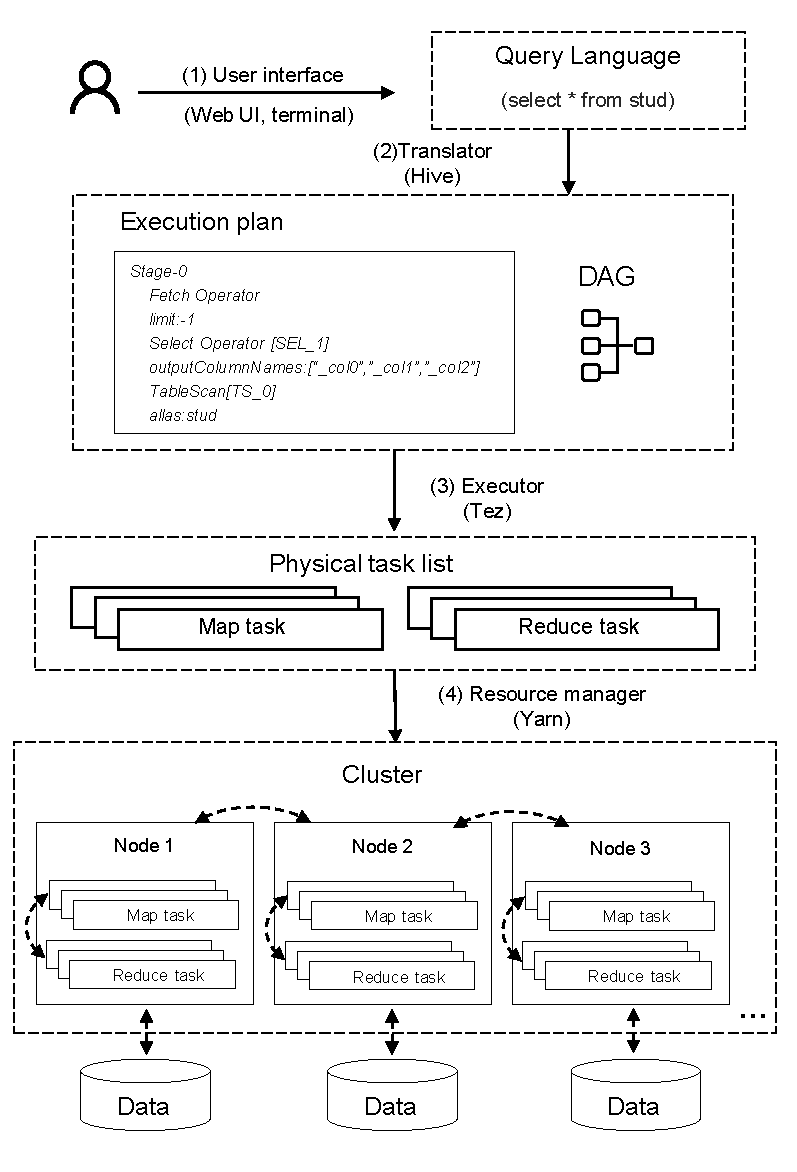
\includegraphics[width=0.42\textwidth]{figures/background/background.pdf}
	\vspace{-3mm}
	\caption{The query processing workflow of Hive (Hadoop 2.0).}
	\label{fig:architecture}
	\vspace{-3mm}
\end{figure}


As illustrated in Figure~\ref{fig:architecture}, query processing in Hive takes four steps. First, the user issues a query via some interface such as web-based UI or SQL terminal as shown in Figure~\ref{fig:architecture}-(1). Then, Hive uses a cost-based optimizer to optimize the query execution plan (e.g., select the best methods to conduct the scan operators, determine a good order for the join operators and choose the index to use) and obtains a logical execution plan as shown in Figure~\ref{fig:architecture}-(2). The logical exaction plan can contain hundreds of lines that describe the query execution process and will be executed by the computation engine (e.g., Tez). We can model the logical exaction plan as a Directed Acyclic Graph (DAG), in which each \textbf{vertex} corresponds to a sequence of logical operators (such as filter, aggregate and etc.) that conducts some sub-steps of the query. For Tez DAG, a vertex can be either a \textbf{map} vertex or a \textbf{reduce} vertex depending on it conducts map tasks or reduce tasks. The \textbf{edges} in a DAG are directed and model the data movement between vertices. For an edge, we call the source vertex \textbf{producer} vertex and the destination vertex \textbf{consumer} vertex. Note that a producer vertex may connect to multiple consumer vertices and a consumer vertex can take inputs from multiple producer vertices. 
 

%When user issues a query (shown as Figure~\ref{fig:architecture}(1)) through the interface such as a web-based user interface or SQL terminal. 
%Hive uses a cost-based optimizer to optimize the query such as determining the best methods for scan operators, join orders and aggregate operation, and then translate it as the logic execution plan shown as Figure~\ref{fig:architecture}(2). The logic exaction plan may contains hundreds of lines of description, which describes the execution process as a Directed Acyclic Graph(DAG) that can be processed by the executor(e.g., Tez). 

%A DAG is a collection of vertices and edges. Logically, a \textbf{vertex} consists of a sequence of logical operators(such as filter, aggregate, etc) which describes the execution of a part of the query. Further more, there are two types of vertices in the Tez DAG, \textbf{map} vertex and \textbf{reduce} vertex.  
%In the DAG,  the \textbf{edges} define the data movement between the adjacent vertices. We name of source vertex as the \textbf{producer} vertex and the target vertex as the \textbf{consumer} vertex. Noticed that a producer vertex may connect to multiple consumer vertices and a consumer vertex could be connected by multiple producer vertices.  

%With a given vertex, Tez further creates a set of atomic \textbf{tasks}(shown as Figure~\ref{fig:architecture}(3)). Then these tasks will be dispatched on the physical machines by Yarn, the resource manage tool of Hadoop2.0. A task takes a piece of data as input and execute all operators defined in the corresponding vertex. To ease the analysis of tasks, we define the sub-processes of a task as five steps. For a map task, the steps are \textit{Initialization}, \textit{Input}, \textit{Processor}, \textit{Sink}, \textit{Spill}. For a reduce task, the second step is \textit{Shuffle} instead. Moreover, the data read by a task could come from the local file or producer tasks.

%With the logical DAG, Tez generates the physical execution plan by spawning a set of atomic \textbf{tasks} for each vertex (as shown in Figure~\ref{fig:architecture}-(3)). Then these tasks will be dispatched on the physical machines by Yarn, the resource manage tool of Hadoop2.0. A task takes a piece of data as input and execute all operators defined in the corresponding vertex. To ease the analysis of tasks, we define the sub-processes of a task as five steps. For a map task, the steps are \textit{Initialization}, \textit{Input}, \textit{Processor}, \textit{Sink}, \textit{Spill}. For a reduce task, the second step is \textit{Shuffle} instead. Moreover, the data read by a task could come from the local file or producer tasks.


According to the logical DAG, Tez generates the physical execution plan by spawning a set of atomic \textbf{tasks} for each vertex (as shown in Figure~\ref{fig:architecture}-(3)). These tasks are then dispatched to the physical machines by Yarn as shown in Figure~\ref{fig:architecture}-(4), the resource manager of Hadoop2.0. Each task takes a piece of data as input and executes all the operators in its corresponding DAG vertex. To track the fine-grained execution process of the tasks, we decompose each task into five steps. For a map task, the steps are \textit{Initialize}, \textit{Input}, \textit{Process}, \textit{Sink}, \textit{Spill}. For a reduce task, the second step is \textit{Shuffle} instead of \textit{Input}. Note that the data read by a task could come from its local file or remote producer tasks.



